\documentclass[11pt]{article}
\usepackage{iftex}
\ifPDFTeX
  \usepackage[T1]{fontenc}
  \usepackage[utf8]{inputenc}
  \usepackage{lmodern}
\else
  \usepackage{fontspec}
\fi
\usepackage{amsmath}
\usepackage{lipsum}
\usepackage{pgfplots}
\pgfplotsset{compat=1.18}
\usepackage[margin=1in]{geometry}
\title{A plot-heavy paper for the compile benchmark}
\author{Purplelink LLC}
\date{October 2026}
\begin{document}
\maketitle
Edit marker: alpha.

\lipsum[1-3]
\begin{figure}[ht]
\centering
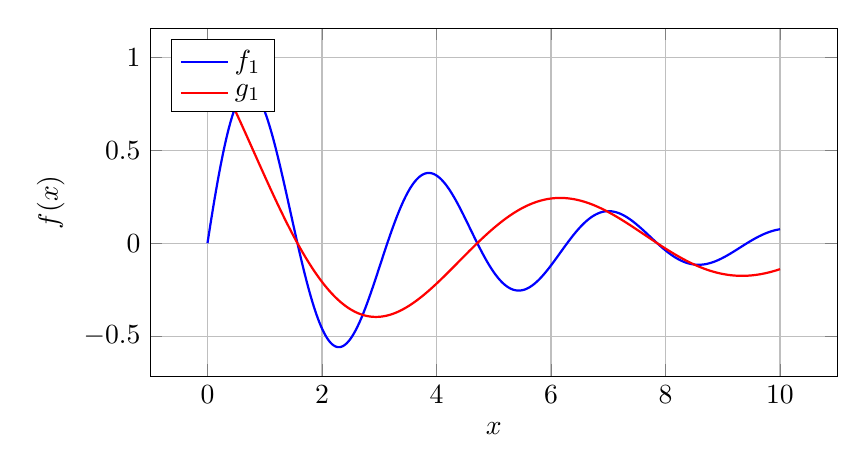
\begin{tikzpicture}
\begin{axis}[width=0.85\linewidth,height=6cm,xlabel={$x$},ylabel={$f(x)$},grid=major,legend pos=north west]
\addplot[blue,thick,domain=0:10,samples=400] {sin(deg(x*2))*exp(-x/4)};
\addplot[red,thick,domain=0:10,samples=400] {cos(deg(x*1))/(1+x/2)};
\legend{$f_{1}$,$g_{1}$}
\end{axis}
\end{tikzpicture}
\caption{Synthetic curves 1.}
\end{figure}
\lipsum[4]
\begin{figure}[ht]
\centering
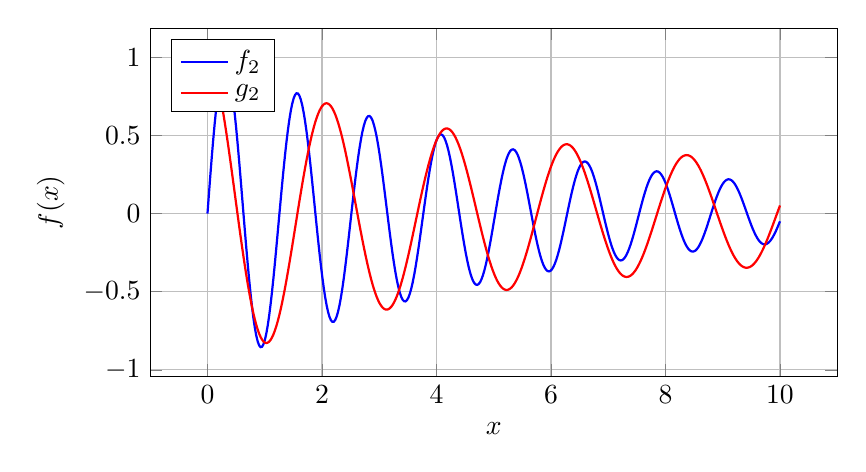
\begin{tikzpicture}
\begin{axis}[width=0.85\linewidth,height=6cm,xlabel={$x$},ylabel={$f(x)$},grid=major,legend pos=north west]
\addplot[blue,thick,domain=0:10,samples=400] {sin(deg(x*5))*exp(-x/6)};
\addplot[red,thick,domain=0:10,samples=400] {cos(deg(x*3))/(1+x/5)};
\legend{$f_{2}$,$g_{2}$}
\end{axis}
\end{tikzpicture}
\caption{Synthetic curves 2.}
\end{figure}
\lipsum[4]
\begin{figure}[ht]
\centering
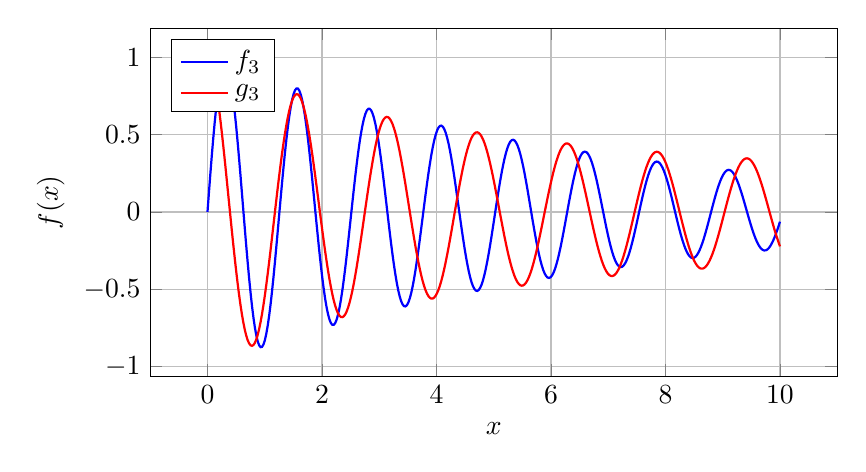
\begin{tikzpicture}
\begin{axis}[width=0.85\linewidth,height=6cm,xlabel={$x$},ylabel={$f(x)$},grid=major,legend pos=north west]
\addplot[blue,thick,domain=0:10,samples=400] {sin(deg(x*5))*exp(-x/7)};
\addplot[red,thick,domain=0:10,samples=400] {cos(deg(x*4))/(1+x/5)};
\legend{$f_{3}$,$g_{3}$}
\end{axis}
\end{tikzpicture}
\caption{Synthetic curves 3.}
\end{figure}
\lipsum[4]
\begin{figure}[ht]
\centering
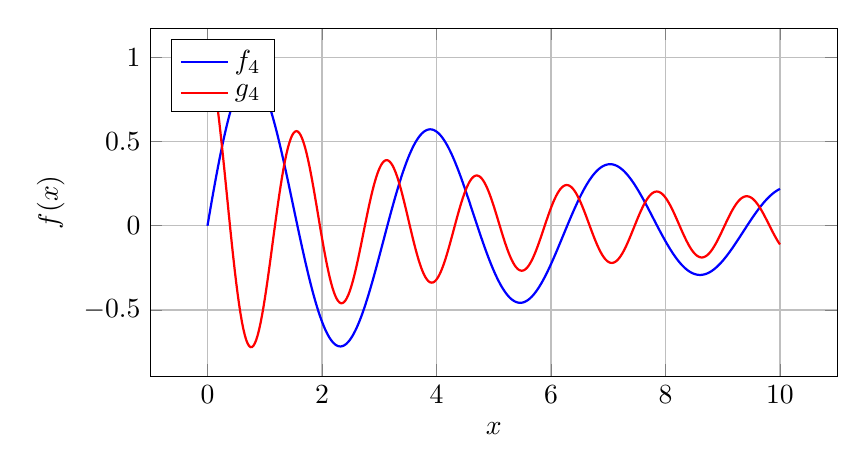
\begin{tikzpicture}
\begin{axis}[width=0.85\linewidth,height=6cm,xlabel={$x$},ylabel={$f(x)$},grid=major,legend pos=north west]
\addplot[blue,thick,domain=0:10,samples=400] {sin(deg(x*2))*exp(-x/7)};
\addplot[red,thick,domain=0:10,samples=400] {cos(deg(x*4))/(1+x/2)};
\legend{$f_{4}$,$g_{4}$}
\end{axis}
\end{tikzpicture}
\caption{Synthetic curves 4.}
\end{figure}
\lipsum[4]
\begin{figure}[ht]
\centering
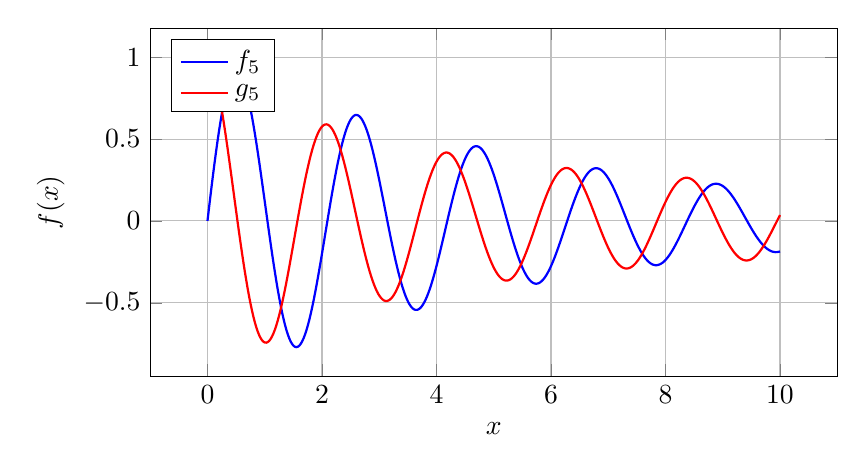
\begin{tikzpicture}
\begin{axis}[width=0.85\linewidth,height=6cm,xlabel={$x$},ylabel={$f(x)$},grid=major,legend pos=north west]
\addplot[blue,thick,domain=0:10,samples=400] {sin(deg(x*3))*exp(-x/6)};
\addplot[red,thick,domain=0:10,samples=400] {cos(deg(x*3))/(1+x/3)};
\legend{$f_{5}$,$g_{5}$}
\end{axis}
\end{tikzpicture}
\caption{Synthetic curves 5.}
\end{figure}
\lipsum[4]
\begin{figure}[ht]
\centering
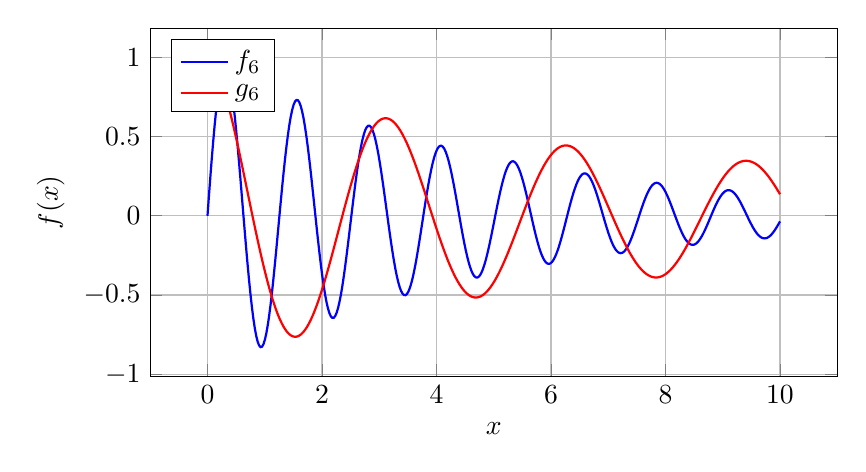
\begin{tikzpicture}
\begin{axis}[width=0.85\linewidth,height=6cm,xlabel={$x$},ylabel={$f(x)$},grid=major,legend pos=north west]
\addplot[blue,thick,domain=0:10,samples=400] {sin(deg(x*5))*exp(-x/5)};
\addplot[red,thick,domain=0:10,samples=400] {cos(deg(x*2))/(1+x/5)};
\legend{$f_{6}$,$g_{6}$}
\end{axis}
\end{tikzpicture}
\caption{Synthetic curves 6.}
\end{figure}
\lipsum[4]
\begin{figure}[ht]
\centering
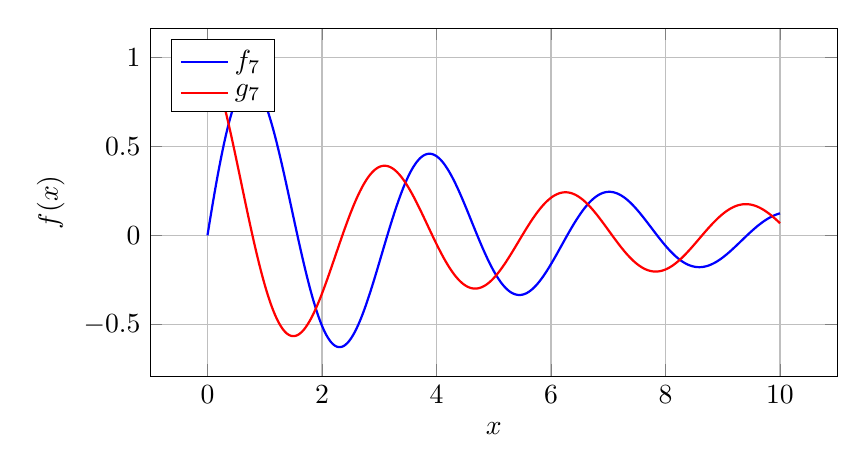
\begin{tikzpicture}
\begin{axis}[width=0.85\linewidth,height=6cm,xlabel={$x$},ylabel={$f(x)$},grid=major,legend pos=north west]
\addplot[blue,thick,domain=0:10,samples=400] {sin(deg(x*2))*exp(-x/5)};
\addplot[red,thick,domain=0:10,samples=400] {cos(deg(x*2))/(1+x/2)};
\legend{$f_{7}$,$g_{7}$}
\end{axis}
\end{tikzpicture}
\caption{Synthetic curves 7.}
\end{figure}
\lipsum[4]
\begin{figure}[ht]
\centering
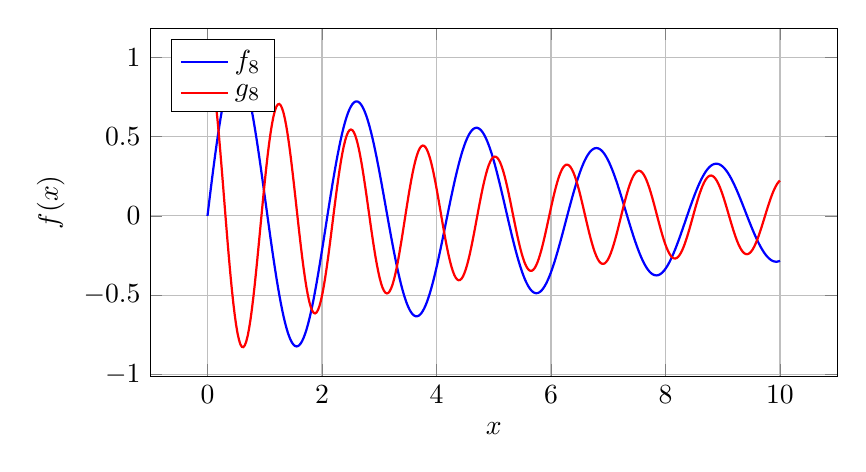
\begin{tikzpicture}
\begin{axis}[width=0.85\linewidth,height=6cm,xlabel={$x$},ylabel={$f(x)$},grid=major,legend pos=north west]
\addplot[blue,thick,domain=0:10,samples=400] {sin(deg(x*3))*exp(-x/8)};
\addplot[red,thick,domain=0:10,samples=400] {cos(deg(x*5))/(1+x/3)};
\legend{$f_{8}$,$g_{8}$}
\end{axis}
\end{tikzpicture}
\caption{Synthetic curves 8.}
\end{figure}
\lipsum[4]
\begin{figure}[ht]
\centering
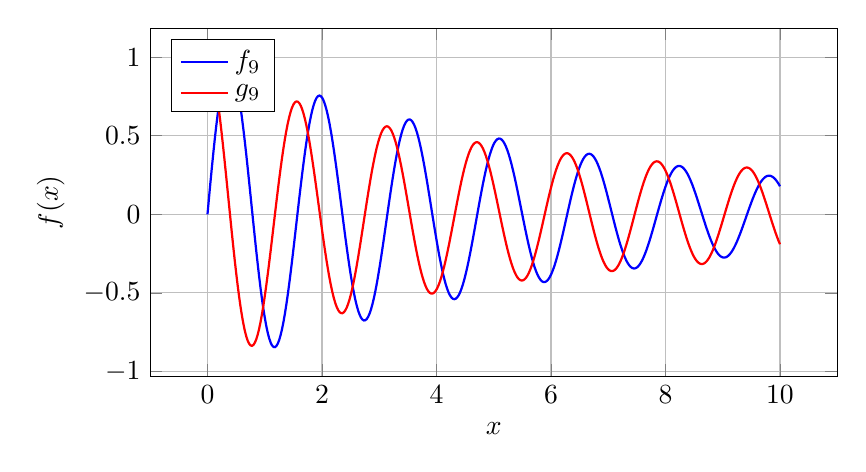
\begin{tikzpicture}
\begin{axis}[width=0.85\linewidth,height=6cm,xlabel={$x$},ylabel={$f(x)$},grid=major,legend pos=north west]
\addplot[blue,thick,domain=0:10,samples=400] {sin(deg(x*4))*exp(-x/7)};
\addplot[red,thick,domain=0:10,samples=400] {cos(deg(x*4))/(1+x/4)};
\legend{$f_{9}$,$g_{9}$}
\end{axis}
\end{tikzpicture}
\caption{Synthetic curves 9.}
\end{figure}
\lipsum[4]
\begin{figure}[ht]
\centering
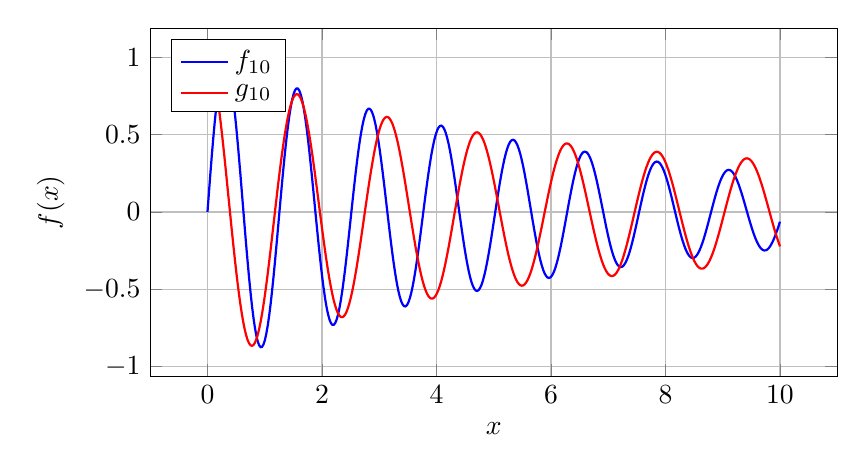
\begin{tikzpicture}
\begin{axis}[width=0.85\linewidth,height=6cm,xlabel={$x$},ylabel={$f(x)$},grid=major,legend pos=north west]
\addplot[blue,thick,domain=0:10,samples=400] {sin(deg(x*5))*exp(-x/7)};
\addplot[red,thick,domain=0:10,samples=400] {cos(deg(x*4))/(1+x/5)};
\legend{$f_{10}$,$g_{10}$}
\end{axis}
\end{tikzpicture}
\caption{Synthetic curves 10.}
\end{figure}
\lipsum[4]
\begin{figure}[ht]
\centering
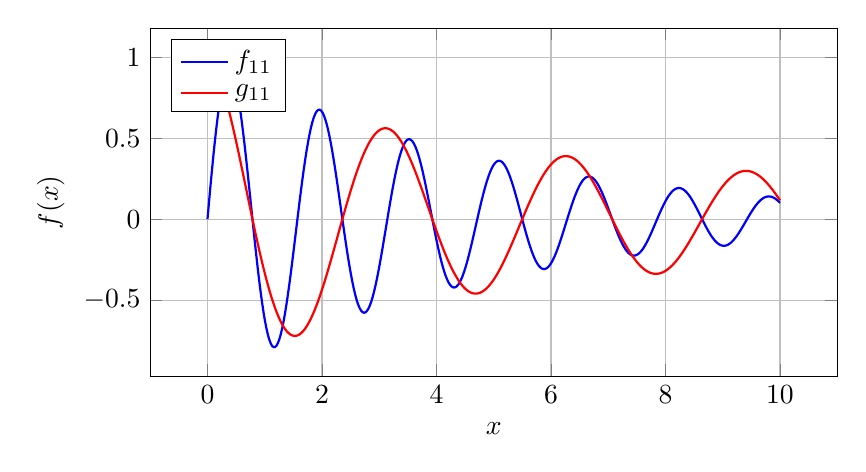
\begin{tikzpicture}
\begin{axis}[width=0.85\linewidth,height=6cm,xlabel={$x$},ylabel={$f(x)$},grid=major,legend pos=north west]
\addplot[blue,thick,domain=0:10,samples=400] {sin(deg(x*4))*exp(-x/5)};
\addplot[red,thick,domain=0:10,samples=400] {cos(deg(x*2))/(1+x/4)};
\legend{$f_{11}$,$g_{11}$}
\end{axis}
\end{tikzpicture}
\caption{Synthetic curves 11.}
\end{figure}
\lipsum[4]
\begin{figure}[ht]
\centering
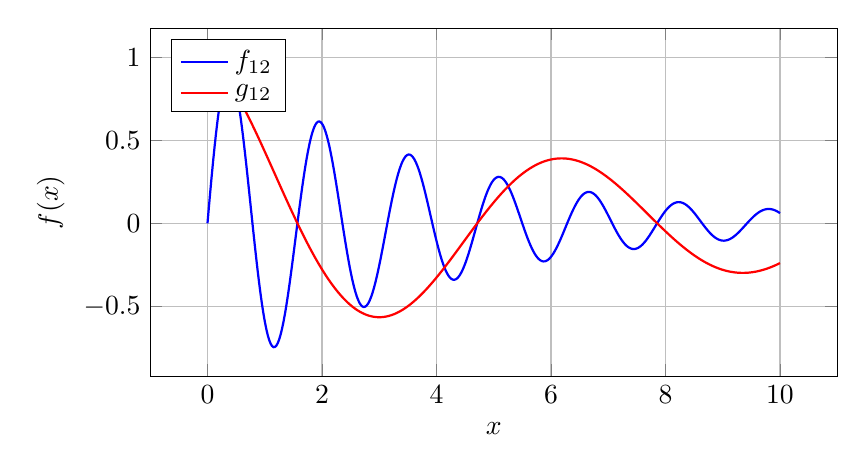
\begin{tikzpicture}
\begin{axis}[width=0.85\linewidth,height=6cm,xlabel={$x$},ylabel={$f(x)$},grid=major,legend pos=north west]
\addplot[blue,thick,domain=0:10,samples=400] {sin(deg(x*4))*exp(-x/4)};
\addplot[red,thick,domain=0:10,samples=400] {cos(deg(x*1))/(1+x/4)};
\legend{$f_{12}$,$g_{12}$}
\end{axis}
\end{tikzpicture}
\caption{Synthetic curves 12.}
\end{figure}
\begin{figure}[ht]
\centering
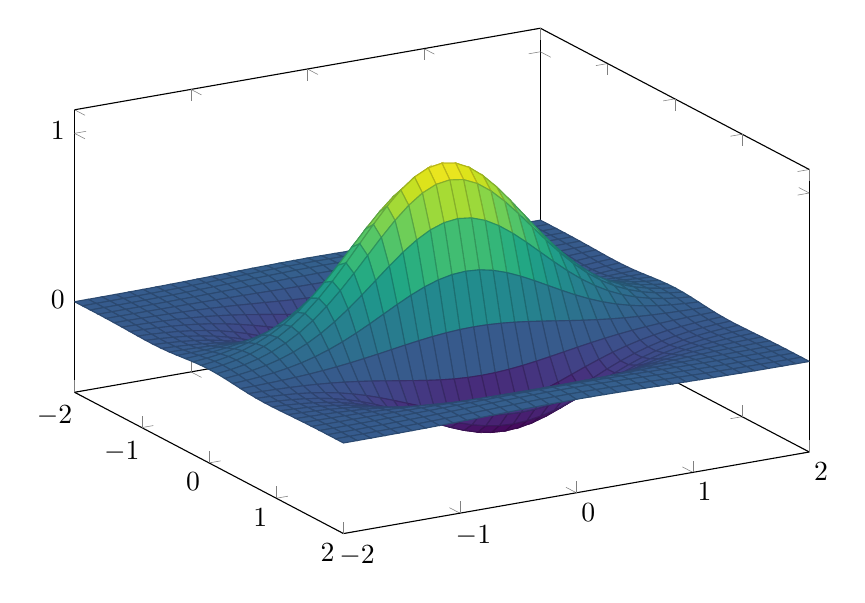
\begin{tikzpicture}
\begin{axis}[view={60}{30},width=0.9\linewidth,height=8cm,colormap/viridis]
\addplot3[surf,domain=-2:2,samples=35] {exp(-x^2-y^2)*cos(deg(3*x))};
\end{axis}
\end{tikzpicture}
\caption{A 35 by 35 surface.}
\end{figure}
\begin{figure}[ht]
\centering
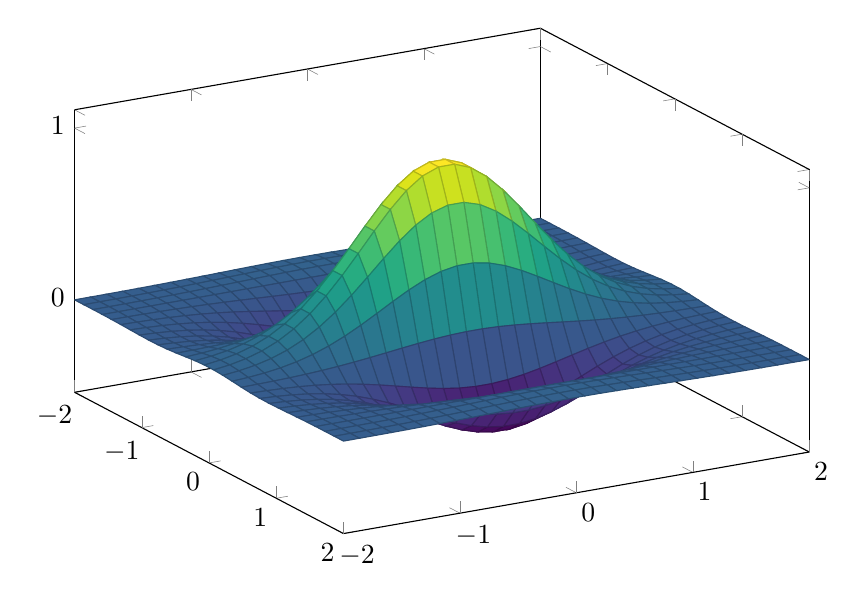
\begin{tikzpicture}
\begin{axis}[view={60}{30},width=0.9\linewidth,height=8cm,colormap/viridis]
\addplot3[surf,domain=-2:2,samples=30] {exp(-x^2-y^2)*cos(deg(3*x))};
\end{axis}
\end{tikzpicture}
\caption{A 30 by 30 surface.}
\end{figure}
\lipsum[5-8]
\end{document}
